%% =============================================================================
%% Sierra Beamer Template - Style Showcase
%% =============================================================================
%% Based on Sierra Template 2025
%% Compile with: xelatex example-presentation.tex
%% (XeLaTeX or LuaLaTeX required for custom Inter fonts)
%% =============================================================================

\documentclass[aspectratio=169]{beamer}

%% Load Sierra theme (with notitlebackground to allow custom background image)
\usetheme[notitlebackground]{Sierra}

%% Additional packages
\usepackage{booktabs}
\usepackage{lipsum}

%% Define Sierra logo for title page (bottom-right corner)
%% Height should roughly match author + institute combined (~1.2cm)
\newcommand{\sierralogo}{%
  
\includegraphics[height=1.2cm]{../assets/sierra-logo-white.png}%
}

%% =============================================================================
%% Presentation Metadata
%% =============================================================================

\title{Presentation Title Goes Here}
\author{Your Name}
\institute{your.email@sierra.ai}
\date{}

%% =============================================================================
%% Document
%% =============================================================================

\begin{document}

%% -----------------------------------------------------------------------------
%% Title Slide (with forest background)
%% -----------------------------------------------------------------------------

{
\usebackgroundtemplate{%
  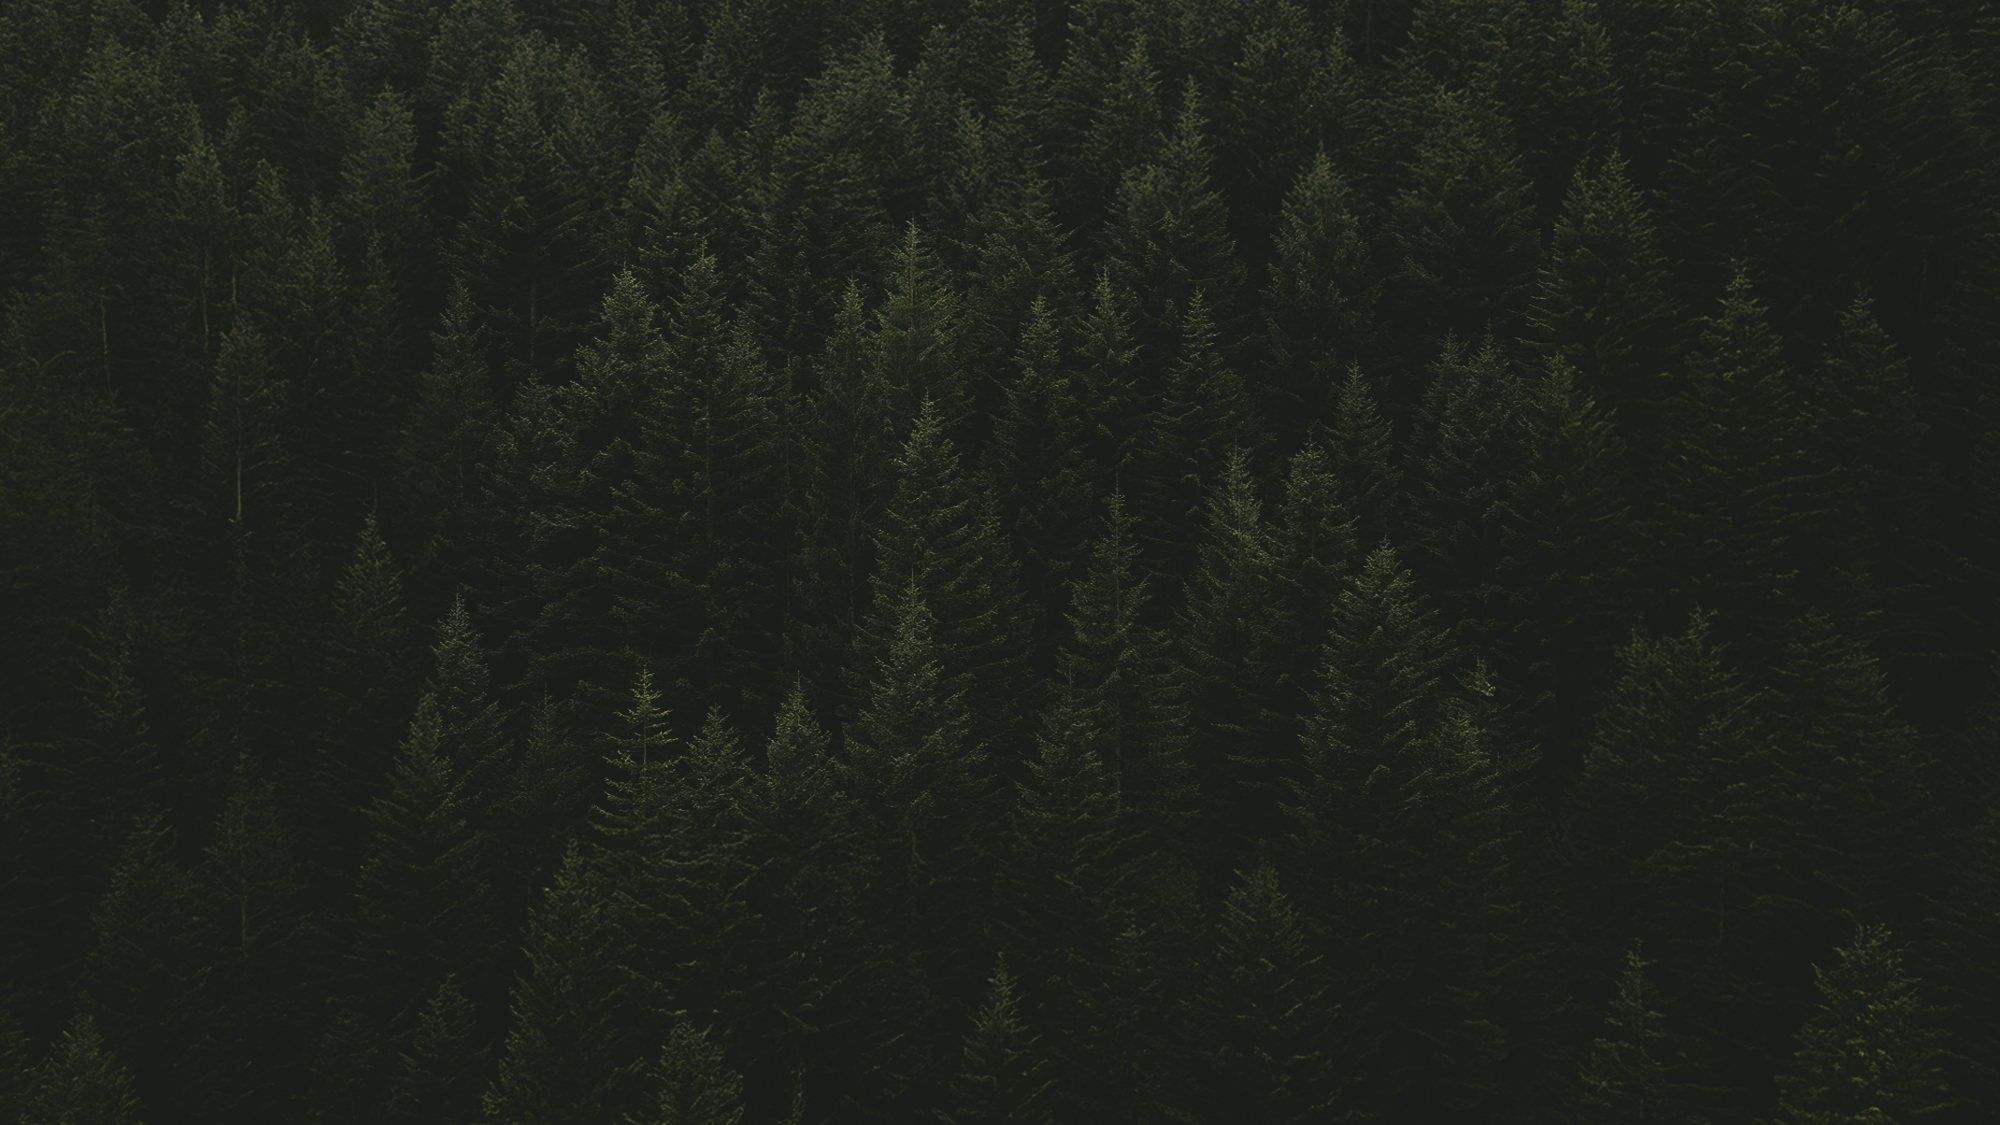
\includegraphics[width=\paperwidth,height=\paperheight]{../assets/sierra-forest-bg.png}%
}
\begin{frame}[plain]
  \titlepage
\end{frame}
}

%% -----------------------------------------------------------------------------
%% Section Slide (with gradient background)
%% -----------------------------------------------------------------------------

{
\usebackgroundtemplate{%
  
\includegraphics[width=\paperwidth,height=\paperheight]{../assets/sierra-gradient-bg.png}%
}
\begin{frame}[plain]
  \centering
  \vfill
  {\fontsize{32}{38}\selectfont\interlight\textcolor{SierraWhite}{Section Title}}
  \vfill
\end{frame}
}

%% -----------------------------------------------------------------------------
%% Basic Content Slide
%% -----------------------------------------------------------------------------

\begin{frame}{Basic Content Slide}
  
  Lorem ipsum dolor sit amet, consectetur adipiscing elit. Sed do eiusmod 
  tempor incididunt ut labore et dolore magna aliqua.
  
  \vspace{1em}
  
  Ut enim ad minim veniam, quis nostrud exercitation ullamco laboris nisi 
  ut aliquip ex ea commodo consequat.
  
\end{frame}

%% -----------------------------------------------------------------------------
%% Bullet Points
%% -----------------------------------------------------------------------------

\begin{frame}{Bullet Points}
  
  \begin{itemize}
    \item First level bullet point with body text
    \item Another first level item
      \begin{itemize}
        \item Second level bullet point
        \item Another second level item
          \begin{itemize}
            \item Third level bullet point
          \end{itemize}
      \end{itemize}
    \item Back to first level
  \end{itemize}
  
\end{frame}

%% -----------------------------------------------------------------------------
%% Numbered Lists
%% -----------------------------------------------------------------------------

\begin{frame}{Numbered Lists}
  
  \begin{enumerate}
    \item First numbered item
      \begin{itemize}
        \item Sub-bullet under numbered item
        \item Another sub-bullet
      \end{itemize}
    \item Second numbered item
    \item Third numbered item
    \item Fourth numbered item
  \end{enumerate}
  
\end{frame}

%% -----------------------------------------------------------------------------
%% Frame with Subtitle
%% -----------------------------------------------------------------------------

\begin{frame}{Frame Title}
  \framesubtitle{With a subtitle underneath}
  
  Lorem ipsum dolor sit amet, consectetur adipiscing elit. Praesent 
  porttitor arcu luctus pulvinar.
  
  \vspace{1em}
  
  \textbf{Bold text} and \textit{italic text} and \alert{alert text} 
  for emphasis.
  
\end{frame}

%% -----------------------------------------------------------------------------
%% Two Columns
%% -----------------------------------------------------------------------------

\begin{frame}{Two Column Layout}
  
  \begin{columns}[T]
    \begin{column}{0.48\textwidth}
      \textbf{Left Column}
      
      Lorem ipsum dolor sit amet, consectetur adipiscing elit.
      
      \begin{itemize}
        \item Point one
        \item Point two
        \item Point three
      \end{itemize}
    \end{column}
    \begin{column}{0.48\textwidth}
      \textbf{Right Column}
      
      Sed do eiusmod tempor incididunt ut labore et dolore magna aliqua.
      
      \begin{itemize}
        \item Item A
        \item Item B
        \item Item C
      \end{itemize}
    \end{column}
  \end{columns}
  
\end{frame}

%% -----------------------------------------------------------------------------
%% Blocks
%% -----------------------------------------------------------------------------

\begin{frame}{Block Styles}
  
  \begin{block}{Standard Block}
    Lorem ipsum dolor sit amet, consectetur adipiscing elit.
  \end{block}
  
  \begin{alertblock}{Alert Block}
    Important warning or highlighted information goes here.
  \end{alertblock}
  
  \begin{exampleblock}{Example Block}
    Example content or code demonstration.
  \end{exampleblock}
  
\end{frame}

%% -----------------------------------------------------------------------------
%% Table
%% -----------------------------------------------------------------------------

\begin{frame}{Tables}
  
  \begin{table}
    \centering
    \begin{tabular}{lcc}
      \toprule
      \textbf{Category} & \textbf{Value A} & \textbf{Value B} \\
      \midrule
      Alpha & 0.85 & 0.72 \\
      Beta & 0.91 & 0.68 \\
      Gamma & 0.78 & 0.81 \\
      Delta & 0.94 & 0.59 \\
      \bottomrule
    \end{tabular}
    \caption{Sample data table with Sierra styling}
  \end{table}
  
\end{frame}

%% -----------------------------------------------------------------------------
%% Statement Slide (Bone/Light variant)
%% -----------------------------------------------------------------------------

{
\setbeamercolor{background canvas}{bg=SierraBone}
\begin{frame}[plain]
  \centering
  \vfill
  {\fontsize{24}{30}\selectfont\interlight\textcolor{SierraCharcoal}{%
    This is a statement slide.\\[0.5em]
    Use it for key messages.%
  }}
  \vfill
\end{frame}
}

%% -----------------------------------------------------------------------------
%% Statement Slide (Green variant)
%% -----------------------------------------------------------------------------

{
\setbeamercolor{background canvas}{bg=SierraGreen}
\begin{frame}[plain]
  \centering
  \vfill
  {\fontsize{24}{30}\selectfont\interlight\textcolor{SierraWhite}{%
    This is a green statement slide.\\[0.5em]
    For emphasis and impact.%
  }}
  \vfill
\end{frame}
}

%% -----------------------------------------------------------------------------
%% Quote Slide (Bone variant)
%% -----------------------------------------------------------------------------

{
\setbeamercolor{background canvas}{bg=SierraBone}
\begin{frame}[plain]
  \centering
  \vfill
  \begin{minipage}{0.75\paperwidth}
    \centering
    {\fontsize{18}{24}\selectfont\interlight\textcolor{SierraCharcoal}{%
      "The best way to predict the future is to invent it."%
    }}
    
    \vspace{1.5em}
    
    {\fontsize{11}{13}\selectfont\intermedium\textcolor{SierraTaupe}{Alan Kay}}
    
    {\fontsize{9}{11}\selectfont\interlight\textcolor{SierraTaupe}{Computer Scientist}}
  \end{minipage}
  \vfill
\end{frame}
}

%% -----------------------------------------------------------------------------
%% Quote Slide (Green variant)
%% -----------------------------------------------------------------------------

{
\setbeamercolor{background canvas}{bg=SierraGreen}
\begin{frame}[plain]
  \centering
  \vfill
  \begin{minipage}{0.75\paperwidth}
    \centering
    {\fontsize{18}{24}\selectfont\interlight\textcolor{SierraWhite}{%
      "The only way to do great work is to love what you do."%
    }}
    
    \vspace{1.5em}
    
    {\fontsize{11}{13}\selectfont\intermedium\textcolor{SierraWhite}{Steve Jobs}}
    
    {\fontsize{9}{11}\selectfont\interlight\textcolor{SierraWhite}{Apple Co-founder}}
  \end{minipage}
  \vfill
\end{frame}
}

%% -----------------------------------------------------------------------------
%% Colors Available
%% -----------------------------------------------------------------------------

\begin{frame}{Available Colors}
  
  \begin{itemize}
    \item \textcolor{SierraCharcoal}{SierraCharcoal} --- Titles, headings
    \item \textcolor{SierraTaupe}{SierraTaupe} --- Body text, bullets
    \item \textcolor{SierraGreen}{SierraGreen} --- Links, accents
    \item \textcolor{SierraDarkGreen}{SierraDarkGreen / SierraForest} --- Dark backgrounds
    \item \textcolor{SierraOrange}{SierraOrange} --- Alerts, highlights
    \item \textcolor{SierraBlueLight}{SierraBlueLight} --- Example blocks (#8BBFF5)
    \item \textcolor{SierraBlue}{SierraBlue} --- Secondary accent
    \item \textcolor{SierraGray}{SierraGray} --- Muted elements
    \item SierraBone / SierraBeige --- Background (\#F6F5F3)
  \end{itemize}
  
\end{frame}

%% -----------------------------------------------------------------------------
%% Thank You Slide (with dusk background and centered logo)
%% -----------------------------------------------------------------------------
%% IMPORTANT: The Sierra logo must ALWAYS be centered at the bottom of this slide.
%% Use TikZ absolute positioning to ensure the logo stays fixed at the bottom center.
%% This guarantees consistent placement regardless of the thank you message length.

{
\usebackgroundtemplate{%
  
\includegraphics[width=\paperwidth,height=\paperheight]{../assets/sierra-dusk-bg.jpg}%
}
\begin{frame}[plain]
  \centering
  \vfill
  
  % Sierra style uses a circular bullet instead of period
  {\fontsize{48}{58}\selectfont\interlight\textcolor{SierraWhite}{Thank you{\large\textbullet}}}
  
  \vfill
  
  % Logo MUST be centered at bottom - use TikZ for absolute positioning
  \begin{tikzpicture}[remember picture,overlay]
    \node[anchor=south, inner sep=0] at ([yshift=0.08\paperheight]current page.south) {%
      
\includegraphics[height=1.5cm]{../assets/sierra-logo-white.png}%
    };
  \end{tikzpicture}
\end{frame}
}

\end{document}
